\section{Materials and Methods}
\label{sec:methods}

Figure~\ref{fig:pipeline-overview} summarises the extraction workflow and its evaluation. The following subsections define the targets, data, processing stages and evaluation protocol.

\begin{figure}[htbp]
\begin{adjustwidth}{-\extralength}{0cm}
\centering
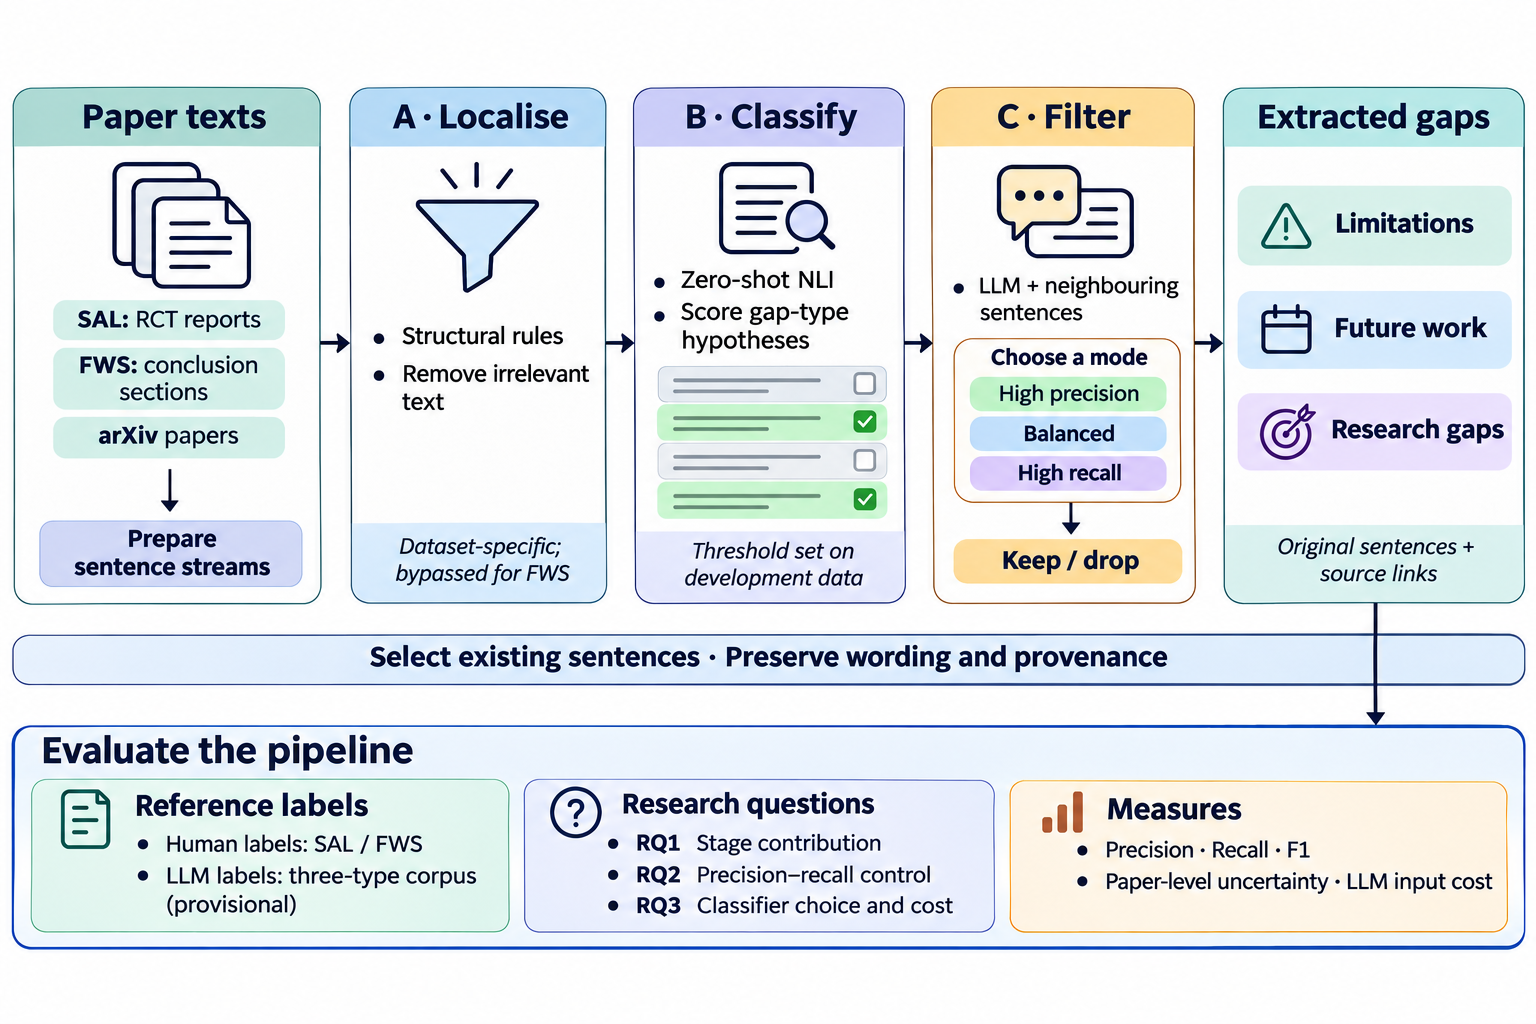
\includegraphics[width=\fulllength]{figures/gap2idea_graphical_abstract_v2.png}
\end{adjustwidth}
\caption{Overview of Gap2Idea. Paper texts are prepared as sentence streams, then processed by structural localisation (A), zero-shot NLI candidate selection (B) and an LLM filter (C). The three filter modes are alternative settings. Outputs retain the original wording and source identifiers. Stage~A is dataset-specific and bypassed for FWS. Human-labelled SAL and FWS evaluate limitations and future work, respectively; evaluation of all three types uses provisional LLM labels. Stage contributions, precision--recall control and classifier choice are assessed alongside LLM input cost.\label{fig:pipeline-overview}}
\end{figure}

\subsection{Task}

The input is the sentence stream of a full paper. The output is the set of sentences that state an author-stated research gap of one of three types:
\begin{itemize}
  \item \textbf{Limitation}: a weakness, caveat, bias, constraint or assumption the authors acknowledge about their own work;
  \item \textbf{Future work}: an explicit direction the authors propose for future research;
  \item \textbf{Research gap}: an unsolved problem, missing capability or open challenge the authors point to in the field or in prior work.
\end{itemize}
Each output is an unmodified source sentence. Scoring is binary at the sentence level: a predicted sentence is correct if its label is any gap type covered by the benchmark. SAL labels only limitations and FWS only future work, so on those benchmarks the funnel targets that one type.

\subsection{Data}

Table~\ref{tab:data} summarises the evaluation data. All splits are by paper.

\begin{table}[htbp]
\caption{Evaluation data. Positives are sentences labelled with a gap type the benchmark covers.\label{tab:data}}
\begin{adjustwidth}{-\extralength}{0cm}
\small
\begin{tabularx}{\fulllength}{@{}>{\raggedright\arraybackslash}p{3.0cm}>{\raggedright\arraybackslash}p{2.3cm}>{\raggedright\arraybackslash}p{2.6cm}rrr>{\raggedright\arraybackslash}X@{}}
\toprule
\textbf{Dataset (split)} & \textbf{Labels} & \textbf{Gap types} & \textbf{Papers} & \textbf{Sentences} & \textbf{Positives} & \textbf{Use}\\
\midrule
SAL (test) & Human & Limitation & 40 & 7968 & 205 & Main evaluation\\
SAL (dev) & Human & Limitation & 40 & 7729 & 180 & Threshold; held-out check\\
FWS (test) & Human & Future work & 209 & 1506 & 220 & Evaluation\\
FWS (dev) & Human & Future work & 418 & 3005 & 418 & Threshold\\
Gold corpus (test) & LLM ensemble & All three & 34 & 11,741 & 664 & Evaluation\\
Gold corpus (validation) & LLM ensemble & All three & 34 & 11,201 & 699 & Design choices; thresholds\\
\bottomrule
\end{tabularx}
\end{adjustwidth}
\end{table}

\paragraph{SAL.} SAL contains 200 RCT publications with sentence-level limitation labels, split into 120 training, 40 development and 40 test papers~\cite{lan2024automatic,salrepo}. We use full papers, not a section-filtered pool. Section types were recovered by matching each sentence to the PubMed Central BioC version of its article, and sentences of fewer than three words were removed; none of the removed test sentences is a limitation. The training split is used only to train the supervised comparison classifiers.

\paragraph{FWS.} The FWS recognition corpus holds conclusion-section sentences from ACL papers labelled as future work or not~\cite{hao2020acl,zhang2023fws,fwsrepo}. Because it contains conclusion sections only, it has no full-paper structure. We use a fixed test sample of 209 papers (1506 sentences) and a development sample of the next 418 papers in the same random order, after removing sentences that appear in an earlier training set of ours. In this corpus every positive sentence is entirely lowercase and almost no negative is (Section~\ref{sec:fws-case}), so we lowercase all FWS text before any processing.

\paragraph{Gold corpus.} We built a three-type corpus of 230 papers and 68,719 sentences: 190 arXiv computer-science and machine-learning papers, converted from PDF with PyMuPDF and split into sentences after removing reference lists, and the 40 SAL test papers with their original sentence boundaries. Two LLMs, Claude Opus~5.5 and Claude Sonnet~5.5, each labelled every sentence of every paper in one call per paper, following a written guideline with the three definitions above. Sentences marked by both with the same type form the high-confidence tier (2960 sentences). The other 1737 candidates marked by only one model, or with different types, were adjudicated by Claude Opus~5.5 with $\pm$3 sentences of context, which confirmed 1502. The final corpus has 4462 gap sentences: 2234 research gaps, 1543 limitations and 685 future-work statements. Agreement between the two labelling models on whether a sentence is a gap was $\kappa = 0.778$~\cite{cohen1960kappa}; this is agreement between models, not with humans. On the 40 SAL papers, the ensemble labelled all but nine of SAL's 205 human-labelled limitations as a gap. SAL labels were not shown to the labelling models. Papers were split into 162 training, 34 validation and 34 test papers. The test split has 664 gaps (220 limitations, 97 future work, 347 research gaps); 28 test papers are arXiv (527 gaps) and 6 are SAL papers (137 gaps). Labelling cost about US\$36.

\subsection{The funnel}

Figure~\ref{fig:funnel} shows the three stages and the gold-test counts at each.

\begin{figure}[htbp]
\begin{adjustwidth}{-\extralength}{0cm}
\centering
\begingroup
\definecolor{funnelInk}{HTML}{183249}
\definecolor{funnelInput}{HTML}{527385}
\definecolor{funnelA}{HTML}{147C87}
\definecolor{funnelB}{HTML}{6553A0}
\definecolor{funnelC}{HTML}{A66916}
\begin{tikzpicture}[
  x=1cm, y=1cm,
  font=\small, text=funnelInk,
  card/.style={rounded corners=5pt, line width=0.7pt},
  title/.style={font=\small\bfseries, anchor=north},
  detail/.style={font=\footnotesize, align=center},
  count/.style={font=\Large\bfseries},
  arr/.style={-{Stealth[length=2.4mm,width=1.8mm]}, line width=1pt, draw=funnelInput}]
% Native vector cards preserve legibility at print resolution.
\draw[card,draw=funnelInput!65,fill=funnelInput!5] (0,0) rectangle (3.1,-4.1);
\draw[card,draw=funnelA!65,fill=funnelA!6] (3.75,0) rectangle (6.85,-4.1);
\draw[card,draw=funnelB!65,fill=funnelB!6] (7.5,0) rectangle (10.6,-4.1);
\draw[card,draw=funnelC!65,fill=funnelC!6] (11.25,0) rectangle (17.6,-4.1);

\node[title,text=funnelInput] at (1.55,-0.23) {INPUT};
\node[title,text=funnelA] at (5.3,-0.23) {A. LOCALISE};
\node[title,text=funnelB] at (9.05,-0.23) {B. CLASSIFY};
\node[title,text=funnelC] at (14.425,-0.23) {C. FILTER};
\node[detail] at (1.55,-0.91) {Full-paper sentences};
\node[detail] at (5.3,-0.91) {Structural rules};
\node[detail] at (9.05,-0.91) {Zero-shot NLI};
\node[detail] at (14.425,-0.91) {LLM with neighbouring sentences};

\node[count,text=funnelInput] at (1.55,-1.67) {11,741};
\node[count,text=funnelA] at (5.3,-1.67) {9604};
\node[count,text=funnelB] at (9.05,-1.67) {2522};
\node[detail] at (1.55,-2.13) {input sentences};
\node[detail] at (5.3,-2.13) {sentences kept};
\node[detail] at (9.05,-2.13) {candidates kept};
\node[count,text=funnelInput] at (1.55,-2.83) {664};
\node[count,text=funnelA] at (5.3,-2.83) {644};
\node[count,text=funnelB] at (9.05,-2.83) {606};
\node[detail] at (1.55,-3.27) {labelled gaps};
\node[detail] at (5.3,-3.27) {labelled gaps retained};
\node[detail] at (9.05,-3.27) {labelled gaps retained};

% Alternative settings, each applied to the same Stage B candidates.
\node[anchor=west,font=\footnotesize\bfseries] at (11.53,-1.52) {Mode};
\node[font=\footnotesize\bfseries] at (15.12,-1.52) {Kept};
\node[font=\footnotesize\bfseries] at (16.78,-1.52) {Gaps};
\fill[rounded corners=3pt,funnelA!13] (11.45,-1.86) rectangle (17.4,-2.43);
\fill[rounded corners=3pt,funnelB!12] (11.45,-2.56) rectangle (17.4,-3.13);
\fill[rounded corners=3pt,funnelC!15] (11.45,-3.26) rectangle (17.4,-3.83);
\node[anchor=west,font=\footnotesize\bfseries,text=funnelA] at (11.6,-2.145) {High precision};
\node[anchor=west,font=\footnotesize\bfseries,text=funnelB] at (11.6,-2.845) {Balanced};
\node[anchor=west,font=\footnotesize\bfseries,text=funnelC] at (11.6,-3.545) {High recall};
\foreach \y/\kept/\gaps in {-2.145/440/381,-2.845/776/529,-3.545/1011/569} {
  \node[font=\small\bfseries] at (15.12,\y) {\kept};
  \node[font=\small\bfseries] at (16.78,\y) {\gaps};
}
\draw[arr] (3.13,-2.05) -- (3.71,-2.05);
\draw[arr] (6.88,-2.05) -- (7.46,-2.05);
\draw[arr] (10.63,-2.05) -- (11.21,-2.05);
\end{tikzpicture}
\endgroup
\end{adjustwidth}
\caption{Sentence selection on the gold test split (34 papers, provisional LLM labels). The first three cards show the input and the sentences retained after Stages~A and~B. Stage~C applies each alternative filter mode to the same candidates; ``Kept'' counts all selected sentences and ``Gaps'' counts selected sentences labelled as gaps. Each stage preserves the original text.\label{fig:funnel}}
\end{figure}

\paragraph{Stage A: localisation.} For SAL, Stage~A keeps sentences in Discussion and Conclusion sections, which retains 203 of 205 test limitations while removing 76.3\% of sentences. For the gold corpus, Stage~A is a rule-based junk filter with no section gate: it drops titles, tables, figure captions, abbreviation lists, competing-interest, author-contribution, funding and supplementary sections where section types are known, bibliography-like strings, and implausible sentences (under 25 characters or six tokens, starting mid-word, dot leaders, or mostly non-letters). A section gate is not used for arXiv papers because their gaps are spread through the body (Section~\ref{sec:discussion}). FWS has no Stage~A: it already consists of conclusion sections, and our junk filter, which rejects sentences that start in lower case, would reject almost all FWS text once it is lowercased.

\paragraph{Stage B: zero-shot NLI classifier.} Each sentence is scored by an NLI cross-encoder, ModernBERT-large fine-tuned on NLI data~\cite{warner2024modernbert,modernbertnli} (revision \texttt{ca476cb9}), used as a zero-shot classifier~\cite{yin2019zeroshot}. The sentence is the premise and a short hypothesis states the gap type: ``This is a limitation.'', ``This is future work.'' or ``This is a research gap.'' The score is the entailment probability divided by the sum of the entailment and contradiction probabilities. On the gold corpus a sentence is a candidate if its maximum score over the three hypotheses reaches a threshold $\tau$, and its predicted type is the hypothesis with the highest score. On SAL only the limitation hypothesis is used, and on FWS only the future-work hypothesis. Inputs are truncated to 256 tokens.

\paragraph{Stage C: LLM filter.} Candidates are sent in reading order, 20 per request, to Qwen3.8-27B (FP8, revision \texttt{017b9c7a}), self-hosted with vLLM~\cite{kwon2023vllm}. This model played no part in making any labels. Each item contains the predicted type, the sentence (up to 400 characters) and its context, the previous and next sentence of the same paper (up to 600 characters). The model returns a keep or drop verdict for each item as JSON constrained by a schema. Decoding uses temperature 0, seed 0 and no reasoning mode. The system prompt (Appendix~\ref{app:prompts}) gives the three definitions, a list of sentence kinds to drop (results, method descriptions, contribution claims, background, citations, captions and similar), and a final instruction that sets the mode:
\begin{itemize}
  \item \textbf{High recall}: when genuinely uncertain, keep the sentence;
  \item \textbf{Balanced}: favour neither keeping nor dropping;
  \item \textbf{High precision}: keep a sentence only if it explicitly states the gap itself, drop general background, motivation, observed outcomes and passing remarks, and when uncertain, drop it.
\end{itemize}
For SAL and FWS the definitions are narrowed to the benchmark's single type, and the other two types are added to the drop list. The wording of each mode is otherwise identical across datasets.

\subsection{How design choices were made}

Because several choices were tuned, we record where each was made.
\begin{itemize}
  \item \textbf{NLI hypotheses.} Hypothesis variants (long definitions, short type names, a single combined hypothesis, adding context, competing negative hypotheses) were compared on one half of the gold validation papers and confirmed on the other half. Short type names were best; context and negative hypotheses hurt.
  \item \textbf{Thresholds.} $\tau$ is the highest value whose overall recall, counting sentences lost in Stage~A, is at least 90\% on development data: gold validation ($\tau = 0.354$), SAL dev ($\tau = 0.7286$) and FWS dev ($\tau = 0.1922$). Values are rounded; at the rounded SAL value one development limitation falls below the threshold, so SAL dev recall before Stage~C is 89.4\% rather than 90.0\%.
  \item \textbf{Stage C model and rubric.} The model, batch size, use of context and the high-recall rubric were chosen during development using 196 candidates from gold test papers; we report gold results with and without these sentences. The balanced and high-precision wording was written after reading false positives from a high-recall run on gold test papers, and was then checked on the gold validation split before any further test run. All three modes were run on every test set and are reported, so no mode was selected by its test score.
  \item \textbf{Held-out check.} The SAL dev papers were used only to set $\tau$; no prompt was written or chosen on them. We run the full funnel on them as a check on unseen papers.
\end{itemize}

\subsection{Comparison systems}

\paragraph{Supervised classifiers on SAL.} We trained eight classifiers on the SAL training split: three fine-tuned encoders, PubMedBERT~\cite{gu2021pubmedbert} (\texttt{BiomedNLP-BiomedBERT-base-uncased-abstract-fulltext}), SciBERT~\cite{beltagy2019scibert} and DistilBERT~\cite{sanh2019distilbert}, each trained for three epochs (learning rate $3\times10^{-5}$, batch 32, class-weighted loss) with a threshold chosen on the SAL dev split; and five frozen sentence encoders~\cite{reimers2019sentencebert,xiao2023cpack} with logistic regression. PubMedBERT was the strongest and serves as the supervised Stage~B comparison; it is also the model family used by Lan et al.~\cite{lan2024automatic}.

\paragraph{Other Stage B options on the gold corpus.} A frozen bge-small encoder~\cite{xiao2023cpack} with a logistic-regression head trained on the gold training split, and the same ModernBERT NLI model with a single long hypothesis covering all gap types (threshold 0.75 chosen on validation).

\paragraph{Whole-paper LLM prompting and published methods.} Comparisons with whole-paper and every-sentence LLM prompting on the same test papers, and reproductions of published methods, are in progress and are not reported in this version.

\subsection{Evaluation}

We report positive-class precision, recall and $F_1$ at the sentence level. The recall denominator is every positive sentence in the test papers, including those removed by Stage~A. Confidence intervals (CIs) are 95\% percentile intervals from 2000 bootstrap resamples of papers~\cite{efron1993bootstrap}, since sentences from one paper are not independent. Comparisons between two systems are paired: both are scored on the same resampled papers, and we report the interval of the difference. LLM input cost is estimated with the \texttt{cl100k\_base} tokenizer~\cite{tiktoken} on the prompts and items exactly as sent; output tokens and Stage~A and B computation are excluded. For comparison we count the input of one whole-paper call (the high-precision prompt followed by the numbered sentences) and of judging every sentence in batches of 20 in the funnel's format. We measured run-to-run stability by repeating the high-recall run on the gold test candidates.

\subsection{Software and use of generative AI}

Experiments used Python with PyTorch, Hugging Face Transformers, sentence-transformers, scikit-learn and vLLM; exact versions are pinned in the repository's lock file. Code is available at the repository listed in the Data Availability Statement. Generative AI is part of the method in two places: Claude Opus~5.5 and Claude Sonnet~5.5 produced the gold-corpus labels, and Qwen3.8-27B is the Stage~C filter. Use of AI assistance in preparing the study and manuscript is declared in the Acknowledgments.
